\documentclass[a4paper]{article}
\usepackage{amsmath}
\addtolength{\hoffset}{-2.25cm}
\addtolength{\textwidth}{4.5cm}
\addtolength{\voffset}{-3.25cm}
\addtolength{\textheight}{5cm}
\setlength{\parindent}{15pt}

\usepackage[unicode=true, colorlinks=false, hidelinks]{hyperref}
\usepackage[utf8]{inputenc}
\usepackage[english, russian]{babel}
\usepackage{mathtext}
\usepackage[T2A, TS1]{fontenc}
\usepackage{microtype} % Slightly tweak font spacing for aesthetics
\usepackage{amsthm, amssymb, amsmath, amsfonts, nccmath}
\usepackage{nicefrac}
\usepackage{epstopdf}
\usepackage[export]{adjustbox}
\usepackage{float} % Improved interface for floating objects
\usepackage{graphicx, multicol} % Enhanced support for graphics
\usepackage{pdfrender,xcolor}
\usepackage{breqn}
\usepackage{mathtools}
\usepackage{titling}
\usepackage{bm}
\usepackage{centernot}
\usepackage[cal=boondoxo,calscaled=.96]{mathalpha}
\usepackage{marvosym, wasysym} % More symbols
\usepackage{rotating} % Rotation tools
\usepackage{censor} % Facilities for controlling restricted text

\usepackage{fancyhdr}
\pagestyle{fancy}
\fancyhead{}\renewcommand{\headrulewidth}{0pt}
\fancyfoot[L]{}
\fancyhead{}
\fancyfoot{}
\fancyfoot[R]{\thepage}
\begin{document}
    \begin{titlepage}
   \begin{center}
       \vspace*{3cm}
       \large{САНКТ-ПЕТЕРБУРГСКИЙ ПОЛИТЕХНИЧЕСКИЙ УНИВЕРСИТЕТ}
       \vspace{0.4 cm}

       \large\textbf{Институт прикладной математики и механики}
       \vspace{0.4 cm}

       \large{Высшая школа прикладной математики и вычислительной физики}

       \vspace{3 cm}
       \normalsize\textbf{Отчет\\ по лабораторной работе №7\\ по дисциплине\\
«Математическая статистика»}
       \vfill
       \begin{flushright}
            \normalsize{Выполнил студент:\\
            Антонов Алексей\\
            группа: 3630102/80201}
            \vskip\medskipamount
            \normalsize{Проверил:

            к.ф.-м.н., доцент\\
            Баженов Александр Николаевич
            }
       \end{flushright}

       \vspace{0.8cm}


       \normalsize{Санкт-Петербург\\2021 г.}

   \end{center}
\end{titlepage}
    \tableofcontents
    \newpage
    \listoftables
    \newpage
    \section {Постановка задачи}
        \noindent Сгенерировать двумерные выборки размерами 20, 60, 100 для нормального двумерного распределения $N(x,y,0,0,1,1,\rho)$. Коэффициент корреляции $\rho$ взять равным 0, 0.5, 0.9. Каждая выборка генерируется 1000 раз и для неё вычисляются: среднее значение, среднее значение квадрата и дисперсия коэффициентов корреляции Пирсона, Спирмена и квадрантного коэффициента корреляции. Повторить все вычисления для смеси нормальных распределений:
        \begin{equation}
        f(x,y) = 0.9N(x,y,0,0,1,1,0.9) + 0.1N(x,y,0,0,10,10,-0.9)
        \end{equation}
        \noindent Изобразить сгенерированные точки на плоскости и нарисовать эллипс равновероятности.

    \section{Теория}
        \subsection{Двумерное нормальное распределение}
            \noindent Двумерная случайная величина $(X,Y)$ называется распределённой нормально (или просто нормальной), если её плотность вероятности определена формулой
            \begin{equation}
                N(x, y, \bar{x}, \bar{y}, \sigma_{x}, \sigma_{y}, \rho) =
                \frac{1}{2\pi\sigma_{x}\sigma_{y}\sqrt{1-\rho^{2}}} \times
                exp{\begin{Bmatrix}
                        -\frac{1}{2(1-\rho^{2})}
                        \begin{bmatrix}
                            \frac{(x-\bar{x})^{2}}{\sigma_{x}^{2}} - 2\rho\frac{(x-\bar{x})(y-\bar{y})}{\sigma_{x}\sigma_{y}} + \frac{(y-\bar{y})^{2}}{\sigma_{y}^{2}}
                        \end{bmatrix}
                    \end{Bmatrix}}
            \end{equation}
            Компоненты $X,Y$ двумерной нормальной случайной величины также распределены нормально с математическими ожиданиями $\bar{x}$,$\bar{y}$ и средними квадратическими отклонениями $\sigma_{x},\sigma_{y}$ соответственно [1, с. 133-134].
            Параметр $\rho$ называется коэффициентом корреляции.


        \subsection{Корреляционный момент (ковариация) и коэффициент корреляции}
            \noindent Корреляционным моментом, иначе ковариацией, двух случайных величин $X$ и $Y$ называется математическое ожидание произведения отклонений этих случайных величин от их математических ожиданий [1, с. 141].
            \begin{equation}
                K = cov(X, Y) = M[(X - \bar{x})(Y - \bar{y})]
                \label{K}
            \end{equation}
            Коэффициентом корреляции $\rho$ двух случайных величин $X$ и $Y$ называется отношение их корреляционного момента к произведению их средних квадратических отклонений:
            \begin{equation}
                \rho = \frac{K}{\sigma_{x}\sigma_{y}}
                \label{ro}
            \end{equation}
            Коэффициент корреляции — это нормированная числовая характеристика, являющаяся мерой близости зависимости между случайными величинами к линейной [1, с. 150].

        \subsection{Выборочные коэффициенты корреляции}
            \subsubsection{Выборочный коэффициент корреляции Пирсона}
                \noindent Пусть по выборке значений ${x_{i},y_{i}}^{n}_{1}$ двумерной с.в. (X,Y ) требуется оценить коэффициент корреляции $\rho = \frac{cov(X,Y)}{\sqrt{DXDY}}$ . Естественной оценкой для $\rho$ служит его статистический аналог в виде выборочного коэффициента корреляции, предложенного К.Пирсоном, —
                \begin{equation}
                    r = \frac{
                        \frac{1}{n}\sum{(x_{i} - \bar{x})(y_{i}-\bar{y})}
                    }{
                    \sqrt{\frac{1}{n}\sum{(x_{i} - \bar{x})^{2}}\frac{1}{n}\sum{(y_{i} - \bar{y})^{2}}}
                    }=\frac{K}{s_{X}s_{Y}},
                    \label{r}
                \end{equation}
                где $K,s^{2}_{X},s^{2}_{Y}$ — выборочные ковариация и дисперсии с.в. $X$ и $Y$ [1, c. 535].


            \subsubsection{Выборочный квадрантный коэффициент корреляции}
                \noindent Кроме выборочного коэффициента корреляции Пирсона, существуют и другие оценки степени взаимосвязи между случайными величинами. К ним относится выборочный квадрантный коэффициент корреляции
                \begin{equation}
                    r_{Q} = \frac{(n_{1} + n_{3}) - (n_{2} + n_{4})}{n},
                    \label{rQ}
                \end{equation}

                \noindent где $n_1, n_2, n_3, n_4 - $ количества точек с координатами $x_i, y_i$, попавшими соответственно в I, II, III, IV квадранты декартовой системы с осями $x'=x-med x$, $y'=y-med y$ и с центром в точке с координатами $(med x,~med y)$



            \subsubsection{Выборочный коэффициент ранговой корреляции Спирмена}
                \noindent На практике нередко требуется оценить степень взаимодействия между качественными признаками изучаемого объекта. Качественным называется признак, который нельзя измерить точно, но который позволяет сравнивать изучаемые объекты между собой и располагать их в порядке убывания или возрастания их качества. Для этого объекты выстраиваются в определённом порядке в соответствии с рассматриваемым признаком. Процесс упорядочения называется ранжированием, и каждому члену упорядоченной последовательности объектов присваивается ранг, или порядковый номер. Например, объекту с наименьшим значением признака присваивается ранг 1, следующему за ним объекту — ранг 2, и т.д. Таким образом, происходит сравнение каждого объекта со всеми объектами изучаемой выборки.
                \newline
                Если объект обладает не одним, а двумя качественными признаками — переменными $X$ и $Y$ , то для исследования их взаимосвязи используют выборочный коэффициент корреляции между двумя последовательностями рангов этих признаков.
                \newline
                Обозначим ранги, соотвествующие значениям переменной $X$, через $u$, а ранги, соотвествующие значениям переменной $Y$, — через $v$.
                \newline
                Выборочный коэффициент ранговой корреляции Спирмена определяется как выборочный коэффициент корреляции Пирсона между рангами $u$,$v$ переменных $X$,$Y$ :
                \begin{equation}
                r_{S} = \frac{
                    \frac{1}{n}\sum{(u_{i} - \bar{u})(v_{i}-\bar{v})}
                }{
                    \sqrt{\frac{1}{n}\sum{(u_{i} - \bar{u})^{2}}\frac{1}{n}\sum{(v_{i} - \bar{v})^{2}}}
                },
                \label{rS}
                \end{equation}
                где $\bar{u} = \bar{v} = \frac{1 + 2 + ... + n}{n} = \frac{n + 1}{2}$ — среднее значение рангов [1, с. 540-541].

        \subsection{Эллипсы рассеивания}
            \noindent Рассмотрим поверхность распределения, изображающую функцию (1). Она имеет вид холма, вершина которого находится над точкой $(\bar{x},\bar{y})$.
            \newline
            В сечении поверхности распределения плоскостями, параллельными оси $ N(x, y, \bar{x}, \bar{y}, \sigma_{x}, \sigma_{y}, \rho)$, получаются кривые, подобные нормальным кривым распределения. В сечении поверхности распределения плоскостями, параллельными плоскости $xOy$, получаются эллипсы. Напишем уравнение проекции такого эллипса на плоскость $xOy$:
            \begin{equation}
                \frac{(x-\bar{x})^{2}}{\sigma_{x}^{2}} -
                2\rho\frac{(x-\bar{x})(y-\bar{y})}{\sigma_{x}\sigma_{y}}+
                \frac{(y-\bar{y})^{2}}{\sigma_{y}^{2}} = const
                \label{ellipse}
            \end{equation}
            Уравнение эллипса \ref{ellipse} можно проанализировать обычными методами аналитической геометрии. Применяя их, убеждаемся, что центр эллипса \ref{ellipse} находится в точке с координатами $(\bar{x},\bar{y})$; что касается направления осей симметрии эллипса, то они составляют с осью Ox углы, определяемые уравнением
            \begin{equation}
                tg(2\alpha) = \frac{2\rho\sigma_{x}\sigma_{y}}{\sigma_{x}^{2} - \sigma_{y}^{2}}
                \label{angle}
            \end{equation}
            Это уравнение дает два значения углов: $\alpha$ и $\alpha_{1}$, различающиеся на $\frac{\pi}{2}$.
            \newline
            Таким образом, ориентация эллипса \ref{ellipse} относительно координатных осей находится в прямой зависимости от коэффициента корреляции $\rho$ системы $(X,Y)$; если величины не коррелированны (т.е. в данном случае и независимы), то оси симметрии эллипса параллельны координатным осям; в противном случае они составляют с координатными осями некоторый угол.
            \newline
            Пересекая поверхность распределения плоскостями, параллельными плоскости $xOy$, и проектируя сечения на плоскость $xOy$ мы получим целое семейство подобных и одинаково расположенных эллипсов с общим центром $(\bar{x},\bar{y})$. Во всех точках каждого из таких эллипсов плотность распределения $ N(x, y, \bar{x}, \bar{y}, \sigma_{x}, \sigma_{y}, \rho)$ постоянна. Поэтому такие эллипсы называются эллипсами равной плотности или, короче эллипсами рассеивания. Общие оси всех эллипсов рассеивания называются главными осями рассеивания [2, с. 193-194].

    \section{Программная реализация}
        Лабораторная работа выполнена на языке Python в среде PyCharm с использованием следующих библиотек:
        \begin{enumerate}
            \item numpy
            \item scipy
            \item matplotlib
        \end{enumerate}

    \section{Результаты}
        \subsection{Выборочные коэффициенты корреляции}
            \begin{table}[H]
                \centering
                \begin{tabular}{| c | c | c | c |}
                    \hline
                    $\rho=$0&$r$&$r_s$&$r_Q$\\ \hline
$E(z)$&0.0004&0.0021&0.0032\\ \hline
$E(z^2)$&0.0548&0.0549&0.0562\\ \hline
$D(z)$&0.0548&0.0549&0.0561\\ \hline
&&&\\ \hline
$\rho = 0.5$&$r$&$r_s$&$r_Q$\\ \hline
$E(z)$&0.4875&0.4608&0.3226\\ \hline
$E(z^2)$&0.2675&0.2456&0.1503\\ \hline
$D(z)$&0.0299&0.0333&0.0462\\ \hline
&&&\\ \hline
$\rho = 0.9$&$r$&$r_s$&$r_Q$\\ \hline
$E(z)$&0.8941&0.8652&0.697\\ \hline
$E(z^2)$&0.802&0.7529&0.5129\\ \hline
$D(z)$&0.0026&0.0043&0.0271\\ \hline

                \end{tabular}{}
                \caption{Двумерное нормальное распределение, n = 20}
                \label{tab:n20}
            \end{table}


            \begin{table}[H]
                \centering
                \begin{tabular}{| c | c | c | c |}
                     \hline
                    $\rho=$0&$r$&$r_s$&$r_Q$\\ \hline
$E(z)$&-0.0013&-0.0053&-0.0081\\ \hline
$E(z^2)$&0.017&0.0163&0.0162\\ \hline
$D(z)$&0.017&0.0163&0.0162\\ \hline
&&&\\ \hline
$\rho = 0.5$&$r$&$r_s$&$r_Q$\\ \hline
$E(z)$&0.4964&0.4733&0.3221\\ \hline
$E(z^2)$&0.2559&0.2346&0.1196\\ \hline
$D(z)$&0.0095&0.0106&0.0159\\ \hline
&&&\\ \hline
$\rho = 0.9$&$r$&$r_s$&$r_Q$\\ \hline
$E(z)$&0.8992&0.8843&0.7114\\ \hline
$E(z^2)$&0.8092&0.7831&0.5146\\ \hline
$D(z)$&0.0007&0.0011&0.0085\\ \hline

                \end{tabular}{}
                \caption{Двумерное нормальное распределение, n = 60}
                \label{tab:n60}
            \end{table}



            \begin{table}[H]
                \centering
                \begin{tabular}{| c | c | c | c |}
                     \hline
                    $\rho=$0&$r$&$r_s$&$r_Q$\\ \hline
$E(z)$&-0.0044&-0.0028&-0.0022\\ \hline
$E(z^2)$&0.0098&0.0095&0.0098\\ \hline
$D(z)$&0.0097&0.0095&0.0098\\ \hline
&&&\\ \hline
$\rho = 0.5$&$r$&$r_s$&$r_Q$\\ \hline
$E(z)$&0.4957&0.4754&0.3303\\ \hline
$E(z^2)$&0.2513&0.2321&0.1176\\ \hline
$D(z)$&0.0055&0.0061&0.0085\\ \hline
&&&\\ \hline
$\rho = 0.9$&$r$&$r_s$&$r_Q$\\ \hline
$E(z)$&0.8999&0.887&0.707\\ \hline
$E(z^2)$&0.8102&0.7873&0.5047\\ \hline
$D(z)$&0.0004&0.0006&0.0048\\ \hline

                \end{tabular}{}
                \caption{Двумерное нормальное распределение, n = 100}
                \label{tab:n100}
            \end{table}


            \begin{table}[H]
                \centering
                \begin{tabular}{| c | c | c | c |}
                    \hline
                    $n=$0&$r$&$r_s$&$r_Q$\\ \hline
$E(z)$&0.4699&0.6639&0.595\\ \hline
$E(z^2)$&0.3736&0.479&0.3879\\ \hline
$D(z)$&0.1527&0.0383&0.0339\\ \hline
&&&\\ \hline
$n = 60$&$r$&$r_s$&$r_Q$\\ \hline
$E(z)$&0.4335&0.6949&0.6279\\ \hline
$E(z^2)$&0.2532&0.4954&0.4045\\ \hline
$D(z)$&0.0653&0.0125&0.0103\\ \hline
&&&\\ \hline
$n = 100$&$r$&$r_s$&$r_Q$\\ \hline
$E(z)$&0.4145&0.6945&0.6319\\ \hline
$E(z^2)$&0.2115&0.4897&0.4051\\ \hline
$D(z)$&0.0398&0.0073&0.0058\\ \hline

                \end{tabular}{}
                \caption{Смесь нормальных распределений}
                \label{tab:mix_normal}
            \end{table}

        \subsection{Эллипсы рассеивания}
             \begin{figure}[H]
                 \centering
                 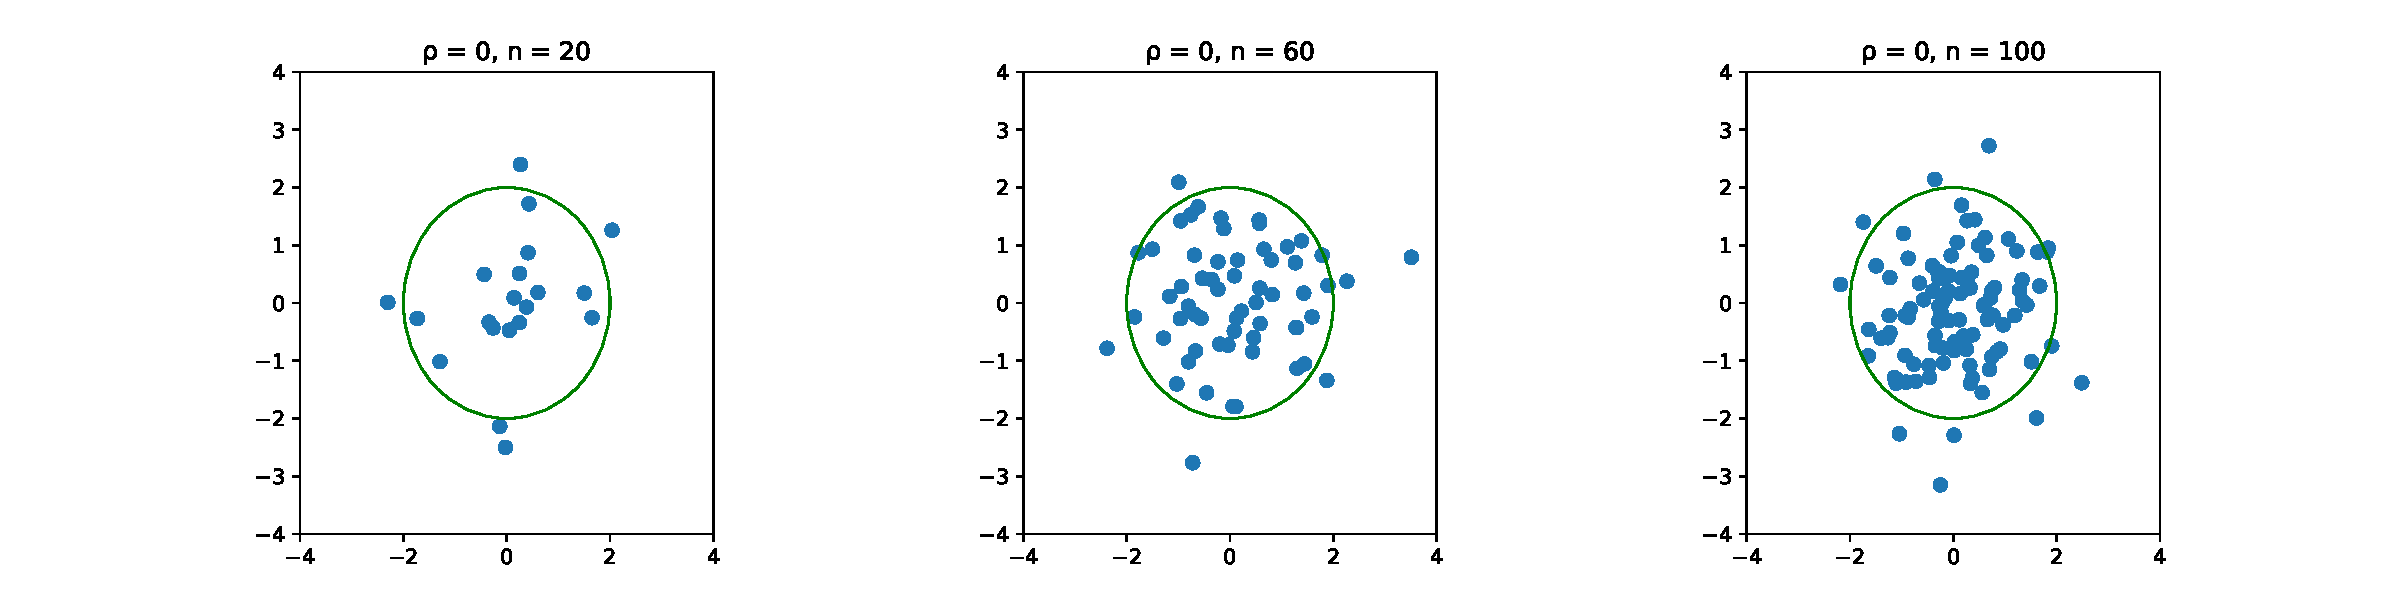
\includegraphics[width = 16cm, height = 4cm]{src/RHO_0}
                 \caption{Двумерное нормальное распределение, $\rho$ = 0}
                 \label{fig:rho_0}
             \end{figure}

             \begin{figure}[H]
                 \centering
                 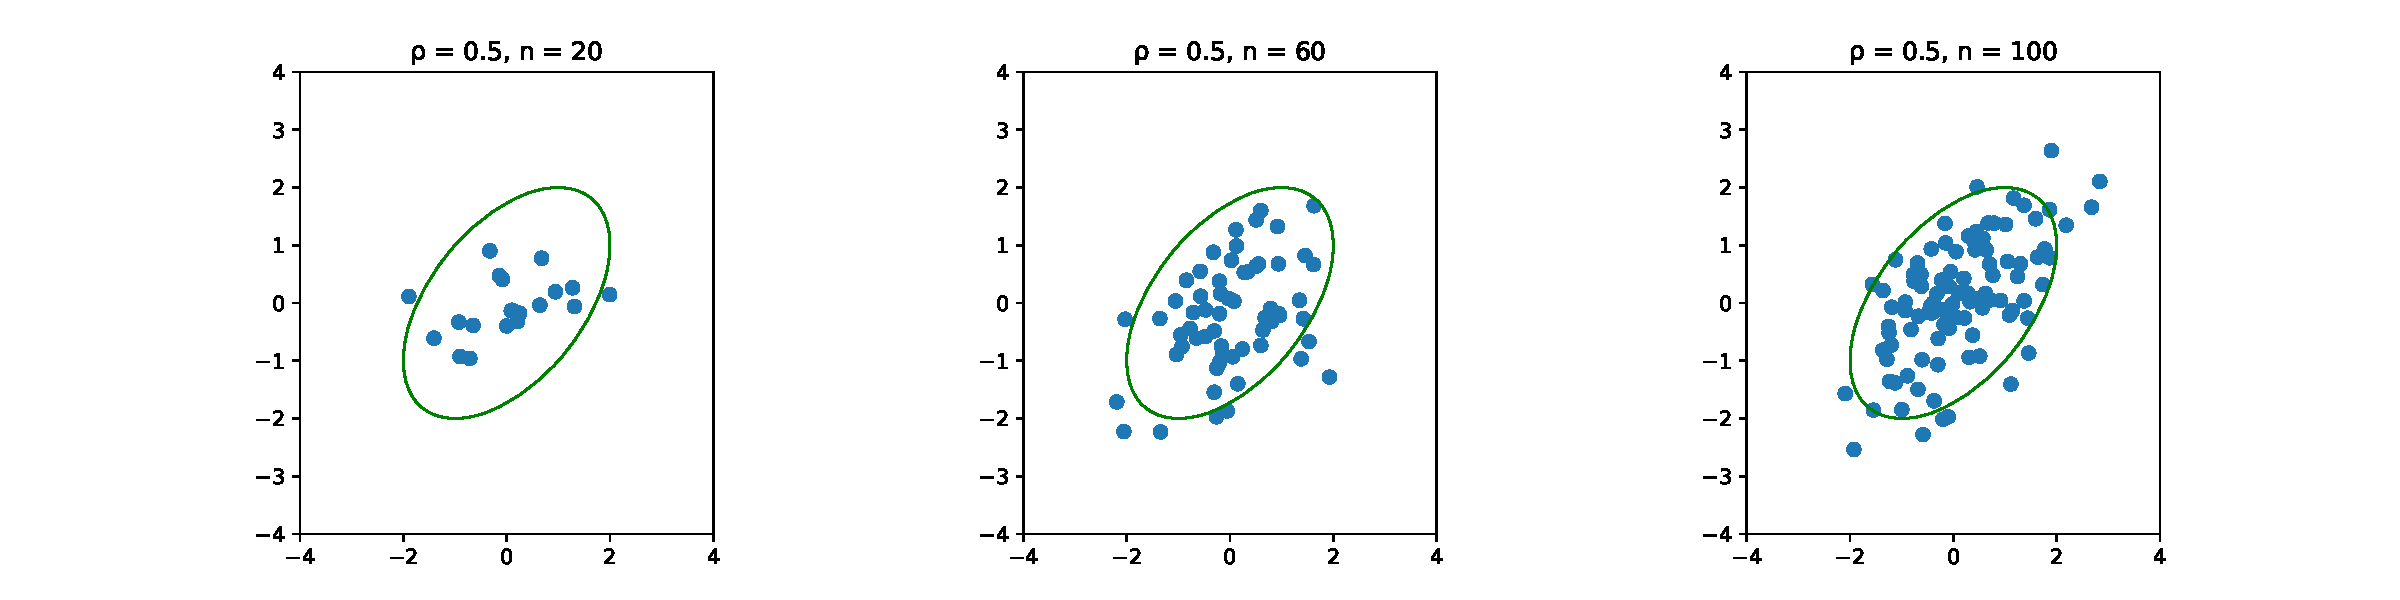
\includegraphics[width = 16cm, height = 4cm]{src/RHO_0.5}
                 \caption{Двумерное нормальное распределение, $\rho$ = 0.5}
                 \label{fig:rho_0_5}
             \end{figure}

             \begin{figure}[H]
                 \centering
                 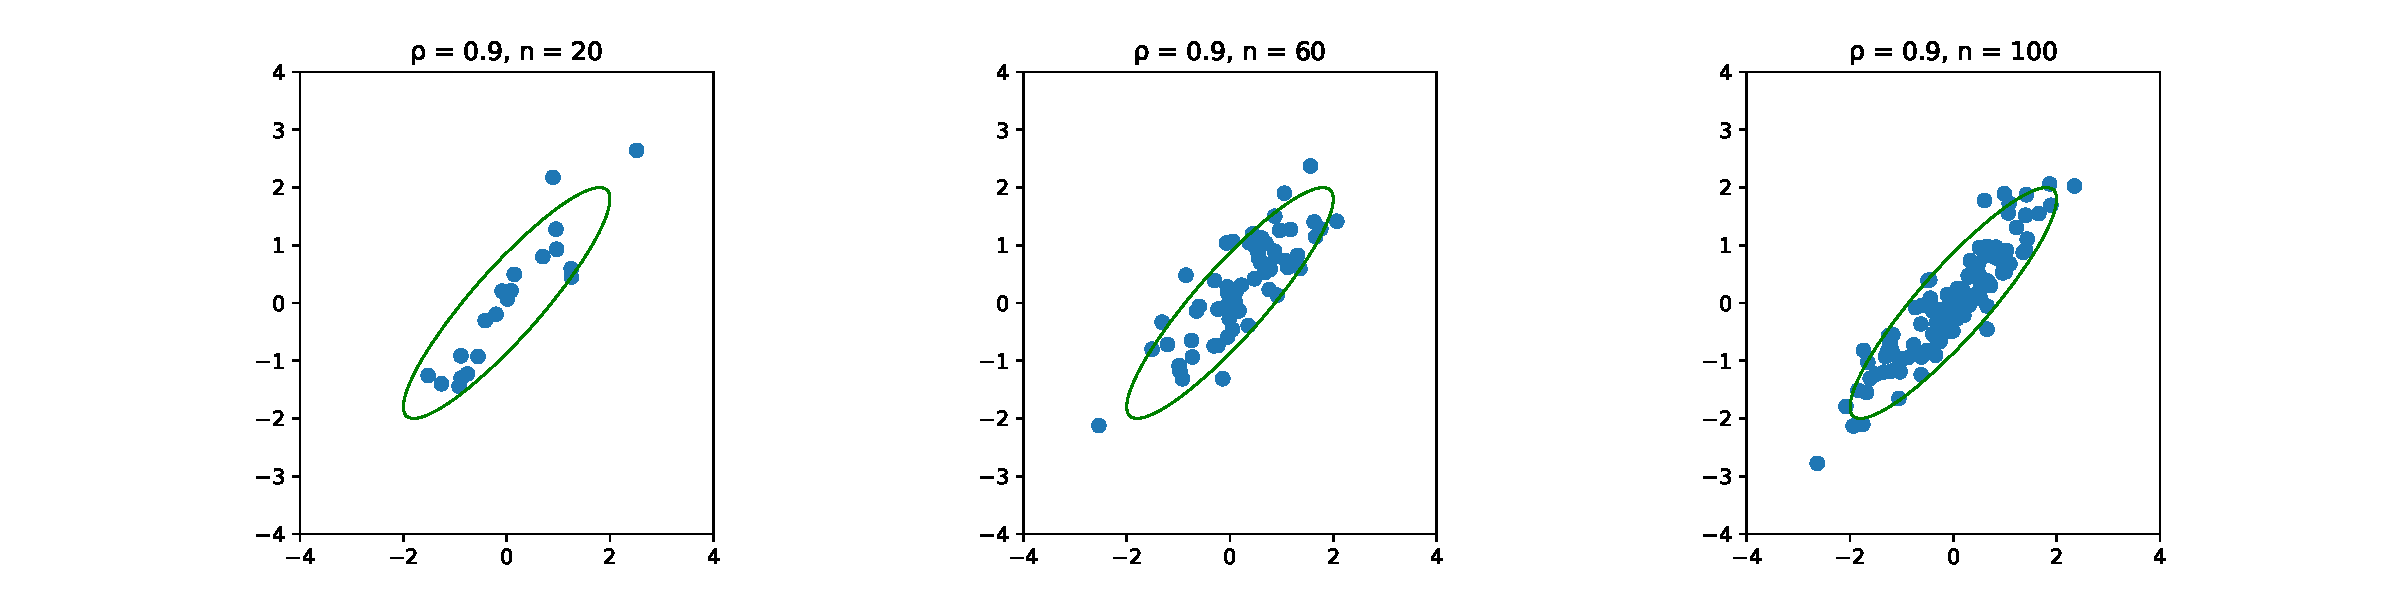
\includegraphics[width = 16cm, height = 4cm]{src/RHO_0.9}
                 \caption{Двумерное нормальное распределение, $\rho$ = 0.9}
                 \label{fig:rho_0_9}
             \end{figure}

    \section{Обсуждение}
        \subsection{Ядерные оценки плотности распределения}
            \noindent Для двумерного нормального распределения дисперсии выборочных коэффициентов корреляции упорядочены следующим образом: $r < r_{S} < r_{Q}$; для смеси распределений получили обратную картину: $r_{Q} < r_{S} < r$.
            \newline
            \noindent Процент попавших элементов выборки в эллипс рассеивания (95$\%$-ная доверительная область) примерно равен его теоретическому значению (95$\%$).

    \section{Приложение}
        С кодом работы и отчета можно ознакомиться по ссылке:\;\url{https://github.com/sqrtyyy/MathStat/tree/master/lab_5}
\end{document}